
%(BEGIN_QUESTION)
% Copyright 2014, Tony R. Kuphaldt, released under the Creative Commons Attribution License (v 1.0)
% This means you may do almost anything with this work of mine, so long as you give me proper credit

Fyll ut tabellen for denne kretsen:

$$\includegraphics[width=15.5cm]{i01179x01.eps}$$

\underbar{file i01179}
%(END_QUESTION)





%(BEGIN_ANSWER)

$$\includegraphics[width=15.5cm]{i01179x02.eps}$$

%(END_ANSWER)





%(BEGIN_NOTES)

Ask your students to identify components in this series-parallel circuit that are guaranteed to share the same voltage, and components that are guaranteed to share the same current, without reference to any calculations.  This is a good exercise in identifying parallel and series interconnections, respectively.

\vskip 10pt

Students often have difficulty formulating a method of solution: determining what steps to take to get from the given conditions to a final answer.  While it is helpful at first for you (the instructor) to show them, it is bad for you to show them too often, lest they stop thinking for themselves and merely follow your lead.  A teaching technique I have found very helpful is to have students come up to the board (alone or in teams) in front of class to write their problem-solving strategies for all the others to see.  They don't have to actually do the math, but rather outline the steps they would take, in the order they would take them.

By having students \underbar{outline their problem-solving strategies}, everyone gets an opportunity to see multiple methods of solution, and you (the instructor) get to see how (and if!) your students are thinking.  An especially good point to emphasize in these ``open thinking'' activities is how to check your work to see if any mistakes were made.

%INDEX% Electronics review: series-parallel circuits

%(END_NOTES)


